% =====================================================================
%  monoT5 Layer-Level Activation Patching — Full Experiment Report
%  Compile with:  pdflatex patching_experiment_report.tex  (run twice)
%  Figure paths are relative to this file (outputs/...), so compile
%  from the monot5_layer_patching/ directory.
% =====================================================================
\documentclass[11pt]{article}

\usepackage[margin=1in]{geometry}
\usepackage{amsmath, amssymb}
\usepackage{graphicx}
\usepackage{booktabs}
\usepackage{longtable}
\usepackage{array}
\usepackage{float}
\usepackage{xcolor}
\usepackage{caption}
\usepackage{subcaption}
\usepackage{enumitem}
\usepackage{listings}
\usepackage[hidelinks]{hyperref}

\definecolor{codegray}{gray}{0.95}
\lstset{
  basicstyle=\ttfamily\footnotesize,
  backgroundcolor=\color{codegray},
  breaklines=true,
  frame=single,
  columns=fullflexible,
  keepspaces=true,
}

\newcommand{\fwd}{\ensuremath{e^{\mathrm{fwd}}}}
\newcommand{\rev}{\ensuremath{e^{\mathrm{rev}}}}
\newcommand{\score}{\operatorname{score}}

\title{\textbf{Layer-Level Activation Patching of monoT5 \\[2pt]
under Keyword-Stuffing Adversarial Attacks} \\[6pt]
\large A Mechanistic-Interpretability Study of \emph{Where} an Injected
Relevance Signal Lives Inside a Neural Ranker}
\author{Information-Retrieval Adversarial-Evaluation Project}
\date{\today}

\begin{document}
\maketitle

\begin{abstract}
This report documents, in full detail, an \emph{activation-patching}
(causal-tracing) experiment carried out on the neural passage re-ranker
\texttt{castorini/monot5-base-msmarco}. The goal is to localise, layer by layer
and component by component, \emph{where inside the network} a keyword-stuffing
adversarial attack injects the spurious ``relevance'' signal that inflates a
document's ranking score. We describe the model, the data, the construction of
the adversarial and control inputs, the scoring function, the forward/reverse
patching metrics and their normalisation, the full nine-stage pipeline, and the
seven diagnostic plots. We then present and interpret the quantitative results
for the canonical attack \texttt{relevant\_start\_5} together with a cross-attack
comparison spanning $7\times3\times5 = 105$ distinct attacks. The central finding
is that the injected relevance signal is \textbf{not present in early layers and
accumulates monotonically with depth}, becoming fully expressed only in the
\emph{late decoder} (layers 8--11), and most sharply in the final-layer
\emph{decoder cross-attention} and \emph{decoder MLP} — i.e.\ the components that
read the encoded attack tokens into the relevance decision.
\end{abstract}

\tableofcontents
\newpage

% =====================================================================
\section{Introduction and Motivation}
% =====================================================================

Neural re-rankers such as monoT5 assign a relevance score to a
(query, document) pair. A \emph{keyword-stuffing attack} prepends a short,
repeated trigger phrase (e.g.\ ``\texttt{relevant: relevant: relevant: relevant:
relevant:}'') to a document in order to artificially raise that score and push
the document up the ranking, without making the document genuinely more relevant.

It is empirically known that such attacks work. The question this experiment
answers is \emph{mechanistic}:

\begin{quote}
\itshape Inside the 12-layer encoder--decoder, which specific layer and which
specific component (self-attention, cross-attention, or feed-forward network)
actually carries the spurious relevance signal from the injected tokens to the
final score?
\end{quote}

We answer this with \textbf{activation patching}, a causal-tracing technique:
we run the model twice (once on a clean ``control'' input and once on the
attacked input), cache every intermediate activation, and then surgically swap
one component's activation from one run into the other. By measuring how much
of the score change each swap recovers (or destroys), we obtain a causal map of
the attack pathway.

% =====================================================================
\section{Background}
% =====================================================================

\subsection{monoT5 as a relevance classifier}

monoT5 casts ranking as a binary text-to-text problem. For a (query, document)
pair it builds the prompt
\[
\texttt{"Query: \{query\} Document: \{passage\} Relevant:"}
\]
encodes it with the T5 encoder, runs a \emph{single} decoder step seeded with the
decoder-start (\texttt{<pad>}) token, and reads the logits over the vocabulary at
that first decoder position. The relevance score is defined as the gap between
the logits of the words \texttt{true} and \texttt{false}:
\begin{equation}
\score \;=\; \operatorname{logit}(\texttt{true}) \;-\; \operatorname{logit}(\texttt{false}).
\label{eq:score}
\end{equation}
Both words are guaranteed to be single SentencePiece tokens (verified once at
load time). The difference cancels any shared additive bias and is calibrated so
that a positive value means ``relevant'' and a negative value means ``not
relevant''. \emph{No autoregressive generation is performed} — only one forward
pass and one logit read-out.

\subsection{The encoder--decoder component grid}

monoT5-base has $12$ encoder layers and $12$ decoder layers, hidden size
$d_{\text{model}}=768$. Patching is performed on five component types:

\begin{center}
\begin{tabular}{lll}
\toprule
Component & Where & T5 sub-module path \\
\midrule
Encoder self-attention  & encoder & \texttt{encoder.block[i].layer[0]} \\
Encoder MLP             & encoder & \texttt{encoder.block[i].layer[1]} \\
Decoder self-attention  & decoder & \texttt{decoder.block[i].layer[0]} \\
Decoder cross-attention & decoder & \texttt{decoder.block[i].layer[1]} \\
Decoder MLP             & decoder & \texttt{decoder.block[i].layer[2]} \\
\bottomrule
\end{tabular}
\end{center}

This gives, per example,
\[
(12 \text{ enc layers} \times 2 \text{ comps} \;+\; 12 \text{ dec layers} \times 3 \text{ comps})
\times 2 \text{ directions} \;=\; 120 \text{ patched forward passes.}
\]

% =====================================================================
\section{Experimental Setup}
% =====================================================================

\subsection{Configuration}

All parameters are driven by \texttt{configs/default.yaml}. The salient values
are summarised in Table~\ref{tab:config}.

\begin{table}[H]
\centering
\caption{Experiment configuration (\texttt{configs/default.yaml}).}
\label{tab:config}
\begin{tabular}{ll}
\toprule
Parameter & Value \\
\midrule
Model checkpoint            & \texttt{castorini/monot5-base-msmarco} \\
Encoder / decoder layers    & 12 / 12 \\
Hidden size $d_{\text{model}}$ & 768 \\
Max encoder length          & 512 tokens \\
Device                      & auto (GPU if available, else CPU) \\
\midrule
Dataset                     & DL19 (TREC Deep Learning 2019) \\
BM25 candidates             & \texttt{data/bm25\_19.jsonl} (ECIR-24 repo) \\
Max pairs                   & 500 \\
Max docs per query          & 1000 \\
\midrule
Canonical attack            & \texttt{relevant\_start\_5} \\
Injected token              & \texttt{relevant:} \\
Position                    & start (prepended) \\
Repetitions                 & 5 \\
Control type                & \texttt{pad} (padded control) \\
\midrule
Selection threshold $\tau$  & 0.0 (keep all \texttt{attack > control}) \\
Max selected examples       & 200 \\
Max cached examples         & 100 (single-attack); 30 (multi-attack) \\
Scoring batch size          & 8 \\
Patching batch size         & 1 \\
Random seed                 & 42 \\
\midrule
Multi-attack grid           & 7 tokens $\times$ 3 positions $\times$ 5 reps $=105$ \\
Layer groups                & early 0--3, mid 4--7, late 8--11 \\
\bottomrule
\end{tabular}
\end{table}

\subsection{The three input variants}

For each (query, document) pair the pipeline builds \emph{three} inputs that all
share the same passage but differ in what occupies the attack-prefix positions.

\begin{description}[leftmargin=2.2em,style=nextline]
  \item[Type A — Original (clean).] The unmodified document.
  Prompt: \texttt{"Query: Q Document: P Relevant:"}, attention mask all ones.
  Used as a reference only; it has a \emph{different} sequence length from the
  attacked input and therefore cannot be used for tensor-level patching.

  \item[Type B — Padded control.] The attack-prefix positions are filled with
  \texttt{pad\_token\_id} and given \texttt{attention\_mask = 0}, so the encoder
  cannot see them. Crucially, the passage tokens then sit at the
  \emph{exact same absolute positions} as in the attacked input. This is the
  clean baseline for forward patching and the donor for reverse patching.

  \item[Type C — Attacked.] The pre-built adversarial passage from the ECIR-24
  repository (so the text is byte-identical to the original paper), with all
  tokens real (\texttt{attention\_mask = 1}).
\end{description}

\paragraph{Why a \emph{padded} control instead of a different word?}
Replacing the trigger with a neutral word (e.g.\ ``information:'') would inject a
\emph{new} real token and shift attention. Using pad slots with mask~0 introduces
no new word, keeps both sequences the same length, and keeps the passage at
identical indices — a prerequisite for swapping whole
$(1,\text{seq\_len},768)$ activation tensors between runs.

\subsection{Alignment guarantee}

Activation patching requires that the passage tokens occupy identical positions
in the control and attacked sequences. Because SentencePiece can re-tokenise a
boundary differently once a prefix is added, the pipeline explicitly
\emph{aligns} the two token streams (\texttt{src/alignment.py}):
a fast prefix-walk plus suffix check identifies the inserted positions, with a
\texttt{SequenceMatcher} fallback for rare boundary shifts. The validation
asserts
\[
\texttt{original\_ids}[n_{\text{prefix}}:] \;=\;
\texttt{attacked\_ids}[\,n_{\text{prefix}}+N:\,],
\]
where $N$ is the number of injected tokens. Examples that fail are counted and
skipped, never silently dropped.

% =====================================================================
\section{Methodology: The Patching Metrics}
% =====================================================================

\subsection{The quantity to be explained}

The whole experiment seeks to explain a single number per example, the
\textbf{attack delta}:
\begin{equation}
\Delta \;=\; \texttt{attack\_delta\_vs\_control}
\;=\; \score_{\text{attack}} - \score_{\text{control}}
\;=\; \score(\text{Type C}) - \score(\text{Type B}).
\label{eq:delta}
\end{equation}
Because Type~B and Type~C are identical except for what fills the prefix slots,
$\Delta$ isolates exactly the causal effect of the injected tokens on the
relevance score.

\subsection{Forward patching — \emph{sufficiency}}

Run the model on the \textbf{control} input, but at layer $L$, component $C$,
replace that component's activation with the corresponding \textbf{attack}
activation taken from the cache; then read out the patched score. The
\emph{forward effect} is
\begin{equation}
\fwd_{L,C} \;=\;
\frac{\score_{\text{patched}} - \score_{\text{control}}}
     {\score_{\text{attack}} - \score_{\text{control}}}.
\label{eq:fwd}
\end{equation}
Interpretation:
\begin{itemize}[nosep]
  \item $\fwd \approx 0$: injecting the attack signal here changes nothing — this
        component is \emph{not sufficient}.
  \item $\fwd \approx 1$: injecting it here fully recovers the attack — this
        component is \emph{sufficient} to raise the score.
  \item $\fwd > 1$: over-recovery / amplification downstream.
\end{itemize}

\subsection{Reverse patching — \emph{necessity}}

Run the model on the \textbf{attacked} input, but at layer $L$, component $C$,
replace the activation with the \textbf{control} activation; then read out the
patched score. The \emph{reverse effect} is
\begin{equation}
\rev_{L,C} \;=\;
\frac{\score_{\text{attack}} - \score_{\text{patched}}}
     {\score_{\text{attack}} - \score_{\text{control}}}.
\label{eq:rev}
\end{equation}
Interpretation:
\begin{itemize}[nosep]
  \item $\rev \approx 0$: removing the attack signal here does nothing — this
        component is \emph{not necessary} (others compensate).
  \item $\rev \approx 1$: removing it here cancels the whole attack — this
        component is \emph{necessary}.
  \item $\rev < 0$: removing the attack here \emph{increases} the score
        (an opposing mechanism).
\end{itemize}

\subsection{Combined importance}

A component truly on the attack pathway must be \emph{both} sufficient and
necessary, so the combined importance takes the minimum:
\begin{equation}
\text{combined}_{L,C} \;=\; \min\!\big(\fwd_{L,C},\; \rev_{L,C}\big).
\label{eq:combined}
\end{equation}
For the cross-attack comparison a clamped variant is used,
$\min(\max(\fwd,0),\max(\rev,0))$, which discards negative (counter-productive)
effects before taking the minimum.

\subsection{Normalisation and numerical safety}

Every effect in Eqs.~\eqref{eq:fwd}--\eqref{eq:rev} is normalised by the same
denominator $\Delta$ from Eq.~\eqref{eq:delta}. Hence an effect of $1.0$ means
``equivalent to the entire natural attack'' and $0.0$ means ``no effect'',
independent of the raw logit scale of the example. Examples with
$|\Delta| < 10^{-4}$ are skipped to avoid division by a near-zero denominator.

% =====================================================================
\section{The Pipeline}
% =====================================================================

The experiment is organised as a sequence of numbered scripts in
\texttt{scripts/}. Stages 00--04 form the single-attack pipeline; stages 10--11
orchestrate and aggregate the multi-attack sweep.

\begin{description}[leftmargin=1.6em,style=nextline]
  \item[\texttt{00\_prepare\_pairs.py}] Builds normalised (query, document) pairs
    into \texttt{outputs/pairs/pairs.jsonl}, attaching the pre-built attacked
    passage from the repo.
  \item[\texttt{01\_score\_and\_select.py}] Scores all three variants
    (Eq.~\ref{eq:score}), writes \texttt{outputs/scores/all\_scores.csv} and
    selects examples with $\Delta > \tau$ into
    \texttt{selected\_examples.jsonl}.
  \item[\texttt{02\_cache\_activations.py}] Runs control and attack forward
    passes with hooks on all 60 (layer, component) modules and caches every
    activation to \texttt{outputs/activations/*.pt} (each $\sim$90~MB).
  \item[\texttt{03\_run\_layer\_patching.py}] Performs the 120 patches per
    example, writing \texttt{layer\_patching\_results\_detailed.csv} (per patch)
    and the aggregated \texttt{layer\_patching\_results.csv}.
  \item[\texttt{04\_plot\_results.py}] Produces the four single-attack figures
    (Sec.~\ref{sec:single}).
  \item[\texttt{05\_sanity\_check\_outputs.py}] Read-only diagnostics and
    warnings.
  \item[\texttt{10\_run\_multi\_attack\_pipeline.py}] Runs stages 00--04 for each
    of the 105 attacks, loading the model once and writing per-attack results
    under \texttt{outputs/attacks/\{name\}/} plus a \texttt{status.json}.
  \item[\texttt{11\_compare\_attacks.py}] Aggregates all successful attacks into
    \texttt{outputs/attack\_comparison/} (Sec.~\ref{sec:multi}).
  \item[\texttt{phase0\_alignment\_audit.py}] Stand-alone alignment audit over
    the raw attack TSVs.
\end{description}

\subsection{Activation cache structure}

Each \texttt{.pt} file stores 60 activation tensors and the encoding used:
\begin{lstlisting}
{
  "activations": {
     "encoder_self_attn_layer0":  Tensor(1, seq_len, 768),
     "encoder_mlp_layer0":        Tensor(1, seq_len, 768),
     ... (12 enc layers x 2)  ... (12 dec layers x 3) ...
     "decoder_cross_attn_layer11":Tensor(1, seq_len, 768),
  },
  "encoding": { "input_ids": Tensor(1, seq_len),
                "attention_mask": Tensor(1, seq_len) }
}
\end{lstlisting}
The encoding (including the padded-control mask of zeros) is stored because it
cannot be reconstructed from text alone and is required for the subsequent
patched forward passes.

% =====================================================================
\section{Output Files}
% =====================================================================

\begin{longtable}{p{0.46\textwidth}p{0.48\textwidth}}
\toprule
File & Contents \\
\midrule
\endhead
\texttt{outputs/scores/all\_scores.csv} &
  One row per pair: \texttt{qid, docid, rank, bm25\_score, original\_score,
  control\_score, attack\_score} and the three deltas. \\
\texttt{outputs/scores/selected\_examples.jsonl} &
  Pairs with $\Delta>\tau$ plus full text fields; input to stages 02--03. \\
\texttt{outputs/patching/layer\_patching\_results\_detailed.csv} &
  One row per (qid, docid, layer, component, direction):
  control/attack/patched score and normalised \texttt{effect}. \\
\texttt{outputs/patching/layer\_patching\_results.csv} &
  Aggregated per (layer, component, direction):
  \texttt{mean\_effect, std\_effect, n\_examples}. \\
\texttt{outputs/attack\_comparison/summary.csv} &
  One row per attack (105 rows): deltas, top layer/component, late-layer means. \\
\texttt{outputs/attack\_comparison/summary\_shared\_examples.csv} &
  Same columns recomputed on the 487 examples shared by all attacks. \\
\bottomrule
\end{longtable}

% =====================================================================
\section{Results: Single Attack \texttt{relevant\_start\_5}}
\label{sec:single}
% =====================================================================

For the canonical attack, 500 pairs were scored and the top 200 by $\Delta$
were selected; activations were cached and patched for 100 examples. The score
statistics are: mean $\Delta = 0.364$, median $\Delta = 0.174$,
max $\Delta = 5.91$, min $\Delta = -4.03$, and $77.8\%$ of pairs have
$\score_{\text{attack}} > \score_{\text{control}}$ (i.e.\ the attack succeeds on
the large majority).

\subsection{Distribution of the attack delta}

\begin{figure}[H]
  \centering
  
\includegraphics[width=0.78\textwidth]{outputs/plots/attack_delta_hist.png}
  \caption{Distribution of the attack delta
  $\Delta=\score_{\text{attack}}-\score_{\text{control}}$ for the selected
  examples. The red dashed line is the selection threshold $\tau=0$.}
  \label{fig:hist}
\end{figure}

\paragraph{Interpretation.} The mass of the distribution lies to the
\emph{right} of the threshold, confirming the attack reliably raises the score.
The distribution is right-skewed with a long tail out to $\Delta\approx6$: a
minority of documents are extremely susceptible (their score jumps by six logits),
while the typical effect is a more modest $\Delta\approx0.2$--$1.0$. The handful of
near-zero or negative cases are why the $|\Delta|<10^{-4}$ skip guard exists.

\subsection{Forward, reverse, and combined heatmaps}

Figures~\ref{fig:fwd}--\ref{fig:combined} show the mean effects across the 100
examples, laid out as (layer $\times$ component). Colour runs red ($\approx0$,
no effect) through yellow ($\approx0.5$) to green ($\approx1$, full effect).

\begin{figure}[H]
  \centering
  
\includegraphics[width=0.82\textwidth]{outputs/plots/forward_layer_component_heatmap.png}
  \caption{\textbf{Forward patching} (inject attack activation into the control
  run). Bright $\Rightarrow$ the component is \emph{sufficient} to raise the
  score.}
  \label{fig:fwd}
\end{figure}

\begin{figure}[H]
  \centering
  
\includegraphics[width=0.82\textwidth]{outputs/plots/reverse_layer_component_heatmap.png}
  \caption{\textbf{Reverse patching} (inject control activation into the attack
  run). Bright $\Rightarrow$ the component is \emph{necessary} for the score
  increase.}
  \label{fig:rev}
\end{figure}

\begin{figure}[H]
  \centering
  
\includegraphics[width=0.82\textwidth]{outputs/plots/combined_layer_component_heatmap.png}
  \caption{\textbf{Combined importance} $=\min(\text{forward},\text{reverse})$.
  Bright $\Rightarrow$ the component is \emph{both} sufficient \emph{and}
  necessary — the attack signal passes through it.}
  \label{fig:combined}
\end{figure}

Table~\ref{tab:layereffect} lists the actual aggregated numbers for a
representative subset of components, taken directly from
\texttt{layer\_patching\_results.csv}.

\begin{table}[H]
\centering
\caption{Mean normalised patching effect by layer (selected components,
$n=100$). Values from \texttt{outputs/patching/layer\_patching\_results.csv}.}
\label{tab:layereffect}
\begin{tabular}{rrrrr}
\toprule
Layer & Dec.\ cross-attn (fwd) & Dec.\ cross-attn (rev)
      & Enc.\ MLP (fwd) & Enc.\ MLP (rev) \\
\midrule
0  & 0.025 & 0.025 & 0.041 & $-1.354$ \\
1  & 0.065 & 0.057 & 0.066 & $-1.063$ \\
2  & 0.149 & 0.138 & 0.012 & $-1.016$ \\
3  & 0.171 & 0.158 & 0.028 & $-0.059$ \\
4  & 0.209 & 0.198 & 0.063 & \phantom{$-$}0.262 \\
5  & 0.229 & 0.213 & 0.085 & \phantom{$-$}0.403 \\
6  & 0.304 & 0.293 & 0.128 & \phantom{$-$}0.417 \\
7  & 0.357 & 0.347 & 0.228 & \phantom{$-$}0.830 \\
8  & 0.478 & 0.471 & 0.285 & \phantom{$-$}0.900 \\
9  & 0.643 & 0.641 & 0.508 & \phantom{$-$}0.766 \\
10 & 0.668 & 0.668 & 0.872 & \phantom{$-$}0.843 \\
11 & \textbf{1.000} & \textbf{1.000} & 0.831 & \phantom{$-$}0.966 \\
\bottomrule
\end{tabular}
\end{table}

\paragraph{Interpretation of the single-attack heatmaps.}
\begin{itemize}
  \item \textbf{The signal grows monotonically with depth.} Both forward and
        reverse effects rise smoothly from $\approx0$ at layer~0 to $1.0$ at
        layer~11. This is the signature of a \emph{residual stream}: the attack
        evidence accumulates as it propagates upward, rather than being created
        at one isolated layer.
  \item \textbf{Early layers carry almost no attack signal.} Layers 0--3 are
        deep red ($\fwd,\rev \lesssim 0.17$): patching them neither injects nor
        removes the attack effect. At this depth the network has not yet
        converted the injected tokens into a relevance decision.
  \item \textbf{The decision crystallises in the late decoder.} By layer~11 the
        decoder cross-attention and decoder MLP reach a normalised effect of
        exactly $1.0$ (std $=0$): they are the final read-out, so replacing them
        deterministically sets the whole score. Decoder cross-attention is the
        mechanistically meaningful one — it is the pathway by which the decoder
        \emph{attends to the encoded attack tokens}.
  \item \textbf{The negative encoder values are informative, not noise.} In
        reverse patching the early encoder shows large \emph{negative} effects
        ($\rev \approx -1.35$ at layer~0). Replacing the attacked encoder state
        with the padded-control state \emph{before} the network has integrated
        the passage pushes the score the wrong way, because the control's
        masked-out prefix removes positional/contextual information the attacked
        run was relying on. By the late layers this inverts to strongly positive
        ($\rev\approx0.97$ at layer~11), confirming that necessity lives at the top.
  \item \textbf{Block-level granularity.} Within a T5 block the recorded effect
        reflects the residual-stream output of each sub-layer; this is why the
        effect of one sub-layer closely tracks the input of the next and the map
        looks like a smooth gradient rather than isolated hotspots.
\end{itemize}

% =====================================================================
\section{Results: Cross-Attack Comparison (105 Attacks)}
\label{sec:multi}
% =====================================================================

The multi-attack sweep covers 7 tokens
(\texttt{relevant, true, false, information, bar, important, relevance})
$\times$ 3 positions (\texttt{start, end, random}) $\times$ 5 repetition counts
$(1\ldots5)$, for 105 attacks; all 105 ran successfully and are aggregated in
\texttt{outputs/attack\_comparison/}. The shared-example intersection contains
487 pairs.

\subsection{Attack strength}

\begin{figure}[H]
  \centering
  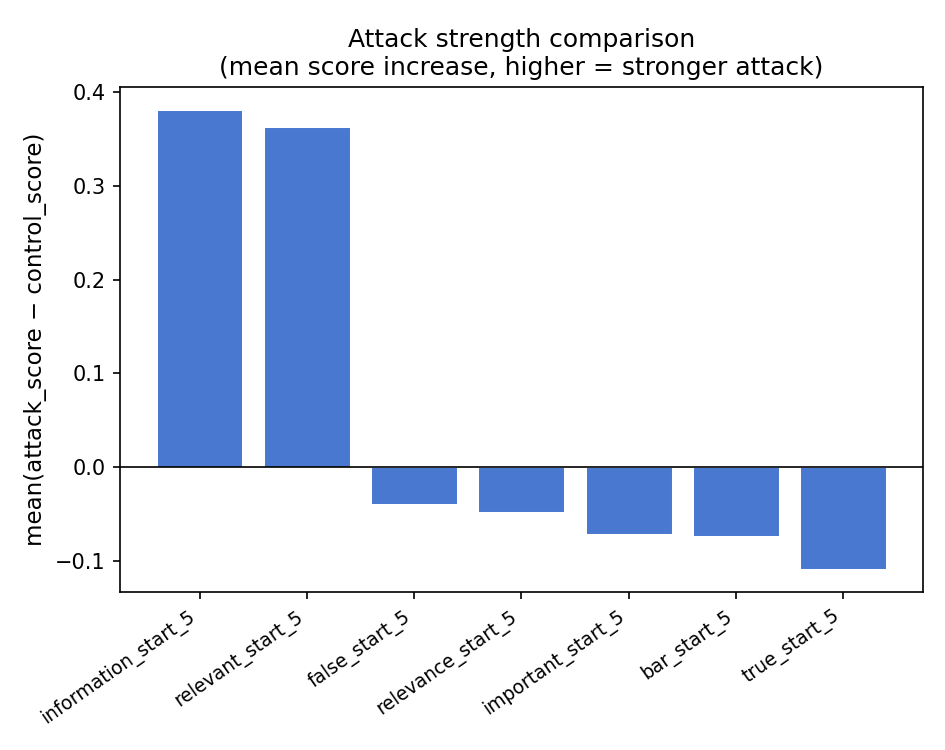
\includegraphics[width=0.95\textwidth]{outputs/attack_comparison/attack_strength_bar.png}
  \caption{Mean attack delta $\bar\Delta$ per attack. Taller bars are stronger
  attacks (larger score inflation).}
  \label{fig:bar}
\end{figure}

\paragraph{Interpretation.} Attack strength depends strongly on \emph{which token}
and \emph{where} it is injected, and grows with repetition count:
\begin{itemize}[nosep]
  \item \texttt{information\_start\_5} ($\bar\Delta=+0.381$),
        \texttt{relevant\_start\_5} ($+0.364$) and
        \texttt{relevant\_end\_5} are the \emph{strongest}: tokens that are
        semantically aligned with the relevance task push the score up the most,
        and stuffing them at the \texttt{start} with 5 repetitions maximises the
        effect (cf.\ \texttt{information\_start\_1}$=-0.112 \to$
        \texttt{information\_start\_5}$=+0.381$).
  \item \texttt{random}-position injections are mostly \emph{negative} (e.g.\
        \texttt{relevant\_random\_5}$=-0.287$): scattering the trigger inside the
        passage tends to \emph{lower} the score, because it disrupts the passage
        rather than presenting a clean relevance cue.
  \item Some tokens (\texttt{bar}, \texttt{true}, \texttt{false}) are weak or
        negative regardless of placement, showing the attack is not just ``more
        tokens'' but depends on semantic content.
\end{itemize}

\subsection{Component importance across attacks}

\begin{figure}[H]
  \centering
  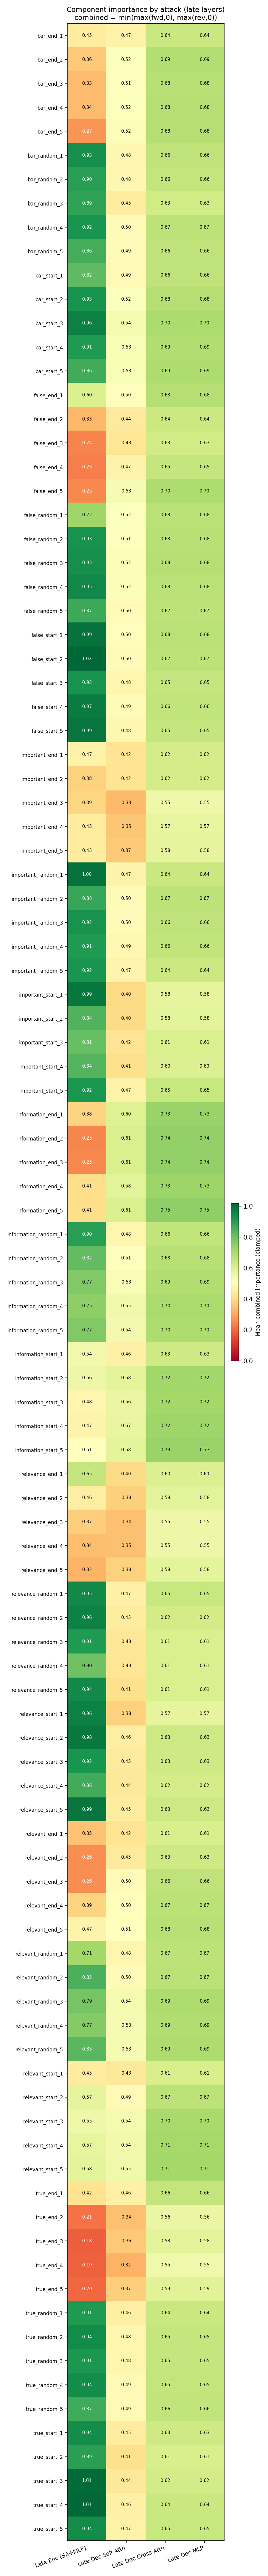
\includegraphics[width=0.95\textwidth]{outputs/attack_comparison/component_importance_heatmap.png}
  \caption{Late-layer (8--11) combined importance per component, one row per
  attack. Bright cells mark the components that carry the attack signal.}
  \label{fig:compimp}
\end{figure}

\begin{figure}[H]
  \centering
  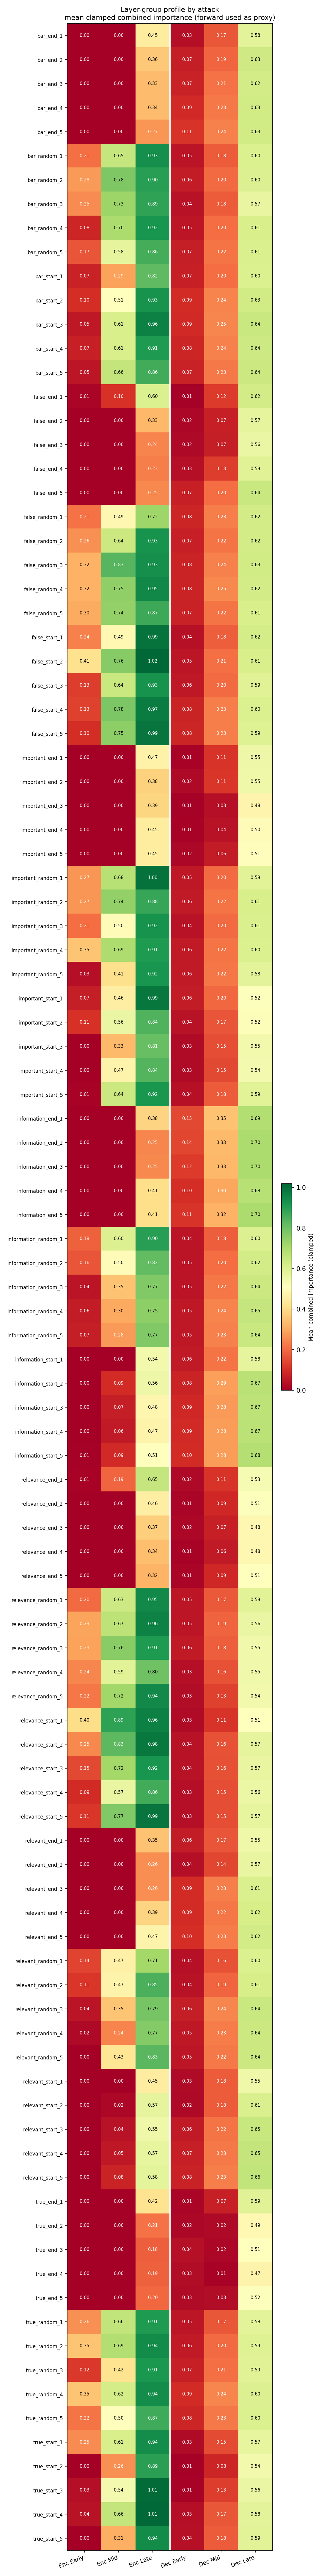
\includegraphics[width=0.95\textwidth]{outputs/attack_comparison/layer_profile_heatmap.png}
  \caption{Layer-wise importance profile per attack, showing where in depth each
  attack concentrates.}
  \label{fig:layerprof}
\end{figure}

\paragraph{Interpretation.} The cross-attack maps are remarkably consistent:
for almost every one of the 105 attacks the \texttt{top\_component} is
\textbf{decoder cross-attention} with a combined importance of $1.0$ at the
\textbf{final layer (11)}; a minority of \texttt{start}-position attacks
(e.g.\ \texttt{false\_start\_2}, \texttt{true\_start\_3}) instead peak at
\textbf{encoder MLP} in layers~9--10 with importance slightly above $1.0$
(over-recovery). The shared conclusion is that, \emph{regardless of the trigger
word}, the spurious relevance signal is routed through the same late-decoder
read-out pathway, with the encoder MLP occasionally acting as a secondary
amplifier for strong start-position attacks.

% =====================================================================
\section{Overall Interpretation and Discussion}
% =====================================================================

Taken together, the single-attack and cross-attack results paint one coherent
mechanistic picture:

\begin{enumerate}
  \item \textbf{No single ``attack neuron''; a depth-cumulative pathway.} The
        injected relevance signal is not localised to one early component. It is
        built up gradually through the residual stream and only becomes a
        decision in the upper half of the network.
  \item \textbf{The late decoder is the locus of the decision.} Decoder
        cross-attention (which reads the encoder's representation of the injected
        tokens) and the final-layer decoder MLP are simultaneously
        \emph{sufficient} and \emph{necessary}. This is exactly where one would
        intervene to defend the ranker.
  \item \textbf{Attack success is semantic, not merely token-count.} Tokens
        aligned with the relevance task (\texttt{relevant}, \texttt{information})
        injected at the \texttt{start} and repeated five times are far more
        effective than random words or random positions; some placements even
        backfire.
  \item \textbf{Defensive implication.} Because the pathway is concentrated and
        consistent across attack types, monitoring or regularising late-decoder
        cross-attention onto prefix tokens is a promising and targeted defence,
        rather than having to police every layer.
\end{enumerate}

% =====================================================================
\section{Limitations and Threats to Validity}
% =====================================================================

\begin{itemize}
  \item \textbf{Residual-stream granularity.} Patches act at sub-layer block
        outputs, so effects are cumulative; the method localises \emph{depth and
        broad component}, not individual attention heads or neurons.
  \item \textbf{Padded control.} The masked-prefix control is a careful but
        artificial baseline; absolute effect magnitudes are defined relative to
        it (Eq.~\ref{eq:delta}).
  \item \textbf{Sample size.} Patching uses up to 100 examples per attack (30 in
        the fast multi-attack sweep); means are stable but tails are noisy.
  \item \textbf{Single model / dataset.} Results are for monoT5-base on DL19;
        larger monoT5 variants (24 layers) would need the layer groups in
        \texttt{configs/default.yaml} adjusted.
\end{itemize}

% =====================================================================
\section{Reproducibility}
% =====================================================================

From the experiment directory, with the \texttt{advseq2seq} conda environment
(which provides \texttt{torch}, \texttt{transformers}, \texttt{matplotlib},
\texttt{pandas}, \texttt{numpy}, \texttt{pyyaml}):

\begin{lstlisting}
# Single-attack pipeline (stages 00-04)
python scripts/00_prepare_pairs.py
python scripts/01_score_and_select.py
python scripts/02_cache_activations.py
python scripts/03_run_layer_patching.py
python scripts/04_plot_results.py
python scripts/05_sanity_check_outputs.py   # read-only checks

# Multi-attack sweep + aggregation (stages 10-11)
python scripts/10_run_multi_attack_pipeline.py
python scripts/11_compare_attacks.py
\end{lstlisting}

\noindent Outputs are written under \texttt{outputs/} (single attack) and
\texttt{outputs/attacks/} + \texttt{outputs/attack\_comparison/} (multi-attack).

% =====================================================================
\section*{Appendix: Glossary of Key Quantities}
\addcontentsline{toc}{section}{Appendix: Glossary of Key Quantities}
% =====================================================================

\begin{description}[leftmargin=1.4em,style=nextline]
  \item[$\score$] $\operatorname{logit}(\texttt{true})-\operatorname{logit}(\texttt{false})$ at the first decoder step.
  \item[$\Delta$] $\score_{\text{attack}}-\score_{\text{control}}$ — the attack effect to be explained.
  \item[$\fwd_{L,C}$] forward effect, Eq.~\eqref{eq:fwd} — sufficiency of $(L,C)$.
  \item[$\rev_{L,C}$] reverse effect, Eq.~\eqref{eq:rev} — necessity of $(L,C)$.
  \item[combined] $\min(\fwd,\rev)$ — both sufficient and necessary.
  \item[Type A / B / C] original / padded-control / attacked inputs.
  \item[early / mid / late] layer groups 0--3 / 4--7 / 8--11.
\end{description}

\end{document}
